% vim: set spell spelllang=en tw=100 et sw=4 sts=4 :

\documentclass[a0paper]{tikzposter}

\usepackage{complexity}
\usepackage{wrapfig}
\usepackage{microtype}
\usepackage{tikz}
\usepackage{gnuplot-lua-tikz}
\usepackage{amssymb}
\usepackage{amsmath}
\usepackage{sfmath}

\usepackage{lmodern}
\renewcommand*\familydefault{\sfdefault}
\usepackage[T1]{fontenc}

\title{Between Subgraph Isomorphism and Maximum Common Subgraph}
\author{Ruth Hoffmann, Ciaran McCreesh and Craig Reilly}
\institute{University of Glasgow, Glasgow, Scotland}
\titlegraphic{
\includegraphics[keepaspectratio=true,scale=3.5]{UoG_keyline.pdf}}

\settitle{
    \begin{tikzpicture}
        \node (T) [inner sep=0pt] {\begin{minipage}{\linewidth}
                \color{titlefgcolor}
                {\bfseries \Huge \hspace*{10mm}Between Subgraph Isomorphism and \\
                \hspace*{10mm}Maximum Common Subgraph \par}
                \vspace*{1em}
                {\Large {\bfseries \hspace{10mm}\@author}, \@institute}
        \end{minipage}};

        \node at (T.east) [anchor=center, inner sep=0pt, xshift=-12cm] {\@titlegraphic};
    \end{tikzpicture}
}

% University of Glasgow standard colours
\definecolor{uofguniversityblue}{rgb}{0, 0.219608, 0.396078}

\definecolor{uofgheather}{rgb}{0.356863, 0.32549, 0.490196}
\definecolor{uofgaquamarine}{rgb}{0.603922, 0.72549, 0.678431}
\definecolor{uofgslate}{rgb}{0.309804, 0.34902, 0.380392}
\definecolor{uofgrose}{rgb}{0.823529, 0.470588, 0.709804}
\definecolor{uofgmocha}{rgb}{0.709804, 0.564706, 0.47451}

\definecolor{uofglawn}{rgb}{0.517647, 0.741176, 0}
\definecolor{uofgcobalt}{rgb}{0, 0.615686, 0.92549}
\definecolor{uofgturquoise}{rgb}{0, 0.709804, 0.819608}
\definecolor{uofgsunshine}{rgb}{1.0, 0.862745, 0.211765}
\definecolor{uofgpumpkin}{rgb}{1.0, 0.72549, 0.282353}
\definecolor{uofgthistle}{rgb}{0.584314, 0.070588, 0.447059}
\definecolor{uofgpillarbox}{rgb}{0.701961, 0.047059, 0}
\definecolor{uofglavendar}{rgb}{0.356863, 0.301961, 0.580392}

\definecolor{uofgsandstone}{rgb}{0.321569, 0.278431, 0.231373}
\definecolor{uofgforest}{rgb}{0, 0.317647, 0.2}
\definecolor{uofgburgundy}{rgb}{0.490196, 0.133333, 0.223529}
\definecolor{uofgrust}{rgb}{0.603922, 0.227451, 0.023529}

\definecolorstyle{UofG}{
}{
    % Background Colors
    \colorlet{backgroundcolor}{uofgsandstone!80!white}
    \colorlet{framecolor}{black}
    % Title Colors
    \colorlet{titlefgcolor}{white}
    \colorlet{titlebgcolor}{uofguniversityblue}
    % Block Colors
    \colorlet{blocktitlebgcolor}{white}
    \colorlet{blocktitlefgcolor}{uofguniversityblue}
    \colorlet{blockbodybgcolor}{white}
    \colorlet{blockbodyfgcolor}{black}
    % Innerblock Colors
    \colorlet{innerblocktitlebgcolor}{uofguniversityblue}
    \colorlet{innerblocktitlefgcolor}{black}
    \colorlet{innerblockbodybgcolor}{uofgsandstone}
    \colorlet{innerblockbodyfgcolor}{black}
    % Note colors
    \colorlet{notefgcolor}{black}
    \colorlet{notebgcolor}{uofgrust}
    \colorlet{noteframecolor}{red}
}

\usetheme{Autumn}
\usecolorstyle{UofG}

\tikzposterlatexaffectionproofoff

\useblockstyle[bodyverticalshift=-1cm, roundedcorners=1]{Default}

\renewcommand{\Huge}{\fontsize{96}{124}\selectfont}

% Styles for drawings

\tikzset{edge/.style={line width=3pt, color=uofgsandstone}}
\tikzset{ledge/.style={line width=3pt, color=uofgsandstone!40!white}}
\tikzset{hedge/.style={line width=3pt, color=uofgsandstone, dashed}}

\setlength\intextsep{0pt}

\begin{document}
\maketitle

{
    \colorlet{blockbodybgcolor}{uofgcobalt}
    \colorlet{blocktitlebgcolor}{uofgcobalt}
    \block[bodyverticalshift=0cm, bodyinnersep=3mm]{}{
        \centering\begin{minipage}{0.94\textwidth}
    When a small pattern graph does not occur inside a larger target graph, we can ask how to find
    \textbf{``as much of the pattern as possible''} inside the target graph. In general, this is known as the \textbf{maximum
    common subgraph problem}, which is much more computationally challenging in practice than
    \textbf{subgraph isomorphism}. We introduce a restricted alternative, where we ask if all but $k$
    vertices from the pattern can be found in the target graph. This allows for the development of
    slightly weakened forms of certain invariants from subgraph isomorphism which are based upon degree and
    number of paths.  We show that when $k$ is small, weakening the invariants still retains much of
    their effectiveness. We are then able to solve this problem on the standard problem
    instances used to benchmark subgraph isomorphism algorithms, despite these instances being
    too large for current maximum common subgraph algorithms to handle. Finally, by iteratively
    increasing $k$, we obtain an algorithm which is also competitive for the maximum common subgraph
    problem.
        \end{minipage}
    }
}

\bigskip

\begin{columns}
\column{0.5}

\block{Subgraph Isomorphism (Finding Patterns in Graphs)}{
\begin{wrapfigure}[11]{r}{0.46\linewidth}

\begin{center}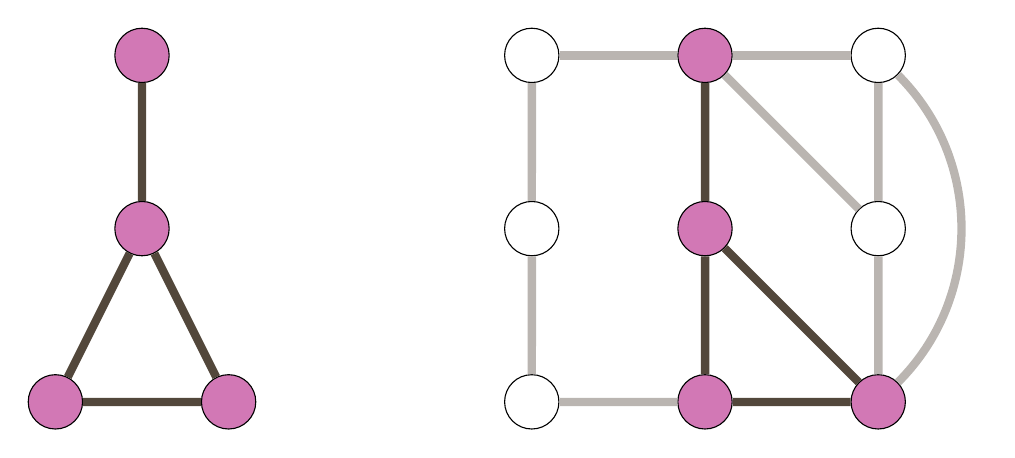
\begin{tikzpicture}[scale=1.1]%{{{
        \node[draw, circle, fill=uofgrose, inner sep=5pt, font=\bfseries] (Na) at (1,  0)
        {\vphantom{0}};
        \node[draw, circle, fill=uofgrose, inner sep=5pt, font=\bfseries] (Nb) at (1, -2)
        {\vphantom{0}};
        \node[draw, circle, fill=uofgrose, inner sep=5pt, font=\bfseries] (Nc) at (0, -4)
        {\vphantom{0}};
        \node[draw, circle, fill=uofgrose, inner sep=5pt, font=\bfseries] (Nd) at (2, -4)
        {\vphantom{0}};

        \draw [edge] (Na) -- (Nb);
        \draw [edge] (Nb) -- (Nc);
        \draw [edge] (Nc) -- (Nd);
        \draw [edge] (Nb) -- (Nd);

        \node[draw, circle, fill=uofgrose, inner sep=5pt, font=\bfseries] (N1) at (7.5,  0) {\vphantom{0}};
        \node[draw, circle, fill=white, inner sep=5pt, font=\bfseries] (N2) at (9.5,  0) {\vphantom{0}};
        \node[draw, circle, fill=uofgrose, inner sep=5pt, font=\bfseries] (N3) at (7.5, -2) {\vphantom{0}};
        \node[draw, circle, fill=white, inner sep=5pt, font=\bfseries] (N4) at (9.5, -2) {\vphantom{0}};
        \node[draw, circle, fill=uofgrose, inner sep=5pt, font=\bfseries] (N5) at (7.5, -4) {\vphantom{0}};
        \node[draw, circle, fill=uofgrose, inner sep=5pt, font=\bfseries] (N6) at (9.5, -4) {\vphantom{0}};
        \node[draw, circle, fill=white, inner sep=5pt, font=\bfseries] (N7) at (5.5,  0) {\vphantom{0}};
        \node[draw, circle, fill=white, inner sep=5pt, font=\bfseries] (N8) at (5.5, -2) {\vphantom{0}};
        \node[draw, circle, fill=white, inner sep=5pt, font=\bfseries] (N9) at (5.5, -4) {\vphantom{0}};

        \draw [ledge] (N1) -- (N2);
        \draw [edge] (N1) -- (N3);
        \draw [ledge] (N1) -- (N4);
        \draw [ledge] (N2) -- (N4);
        \draw [edge] (N3) -- (N5);
        \draw [edge] (N3) -- (N6);
        \draw [ledge] (N4) -- (N6);
        \draw [edge] (N5) -- (N6);
        \draw [ledge] (N2) to [in=45, out=315] (N6);
        \draw [ledge] (N1) -- (N7);
        \draw [ledge] (N5) -- (N9);
        \draw [ledge] (N7) -- (N8);
        \draw [ledge] (N8) -- (N9);
    \end{tikzpicture}\end{center}

    \vspace*{1.5cm}

    \begin{center}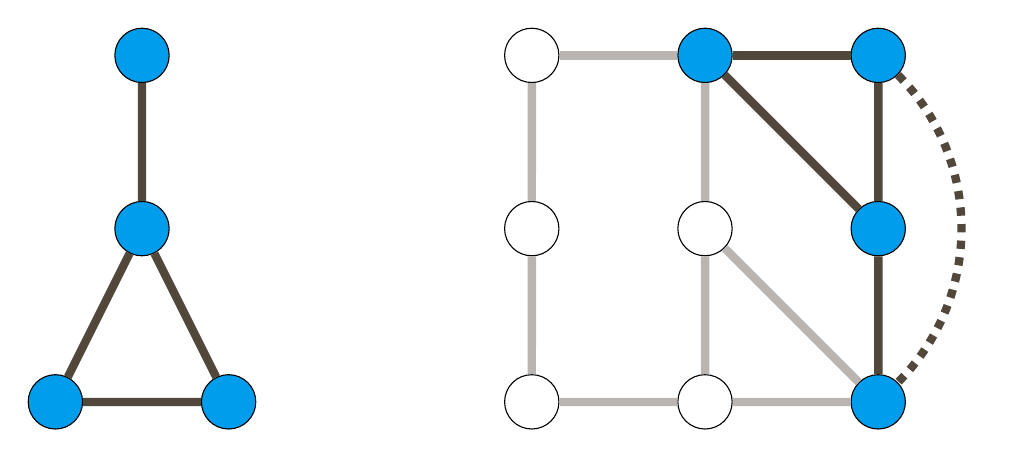
\begin{tikzpicture}[scale=1.1]%{{{
        \node[draw, circle, fill=uofgcobalt, inner sep=5pt, font=\bfseries] (Na) at (1,  0)
        {\vphantom{0}};
        \node[draw, circle, fill=uofgcobalt, inner sep=5pt, font=\bfseries] (Nb) at (1, -2)
        {\vphantom{0}};
        \node[draw, circle, fill=uofgcobalt, inner sep=5pt, font=\bfseries] (Nc) at (0, -4)
        {\vphantom{0}};
        \node[draw, circle, fill=uofgcobalt, inner sep=5pt, font=\bfseries] (Nd) at (2, -4)
        {\vphantom{0}};

        \draw [edge] (Na) -- (Nb);
        \draw [edge] (Nb) -- (Nc);
        \draw [edge] (Nc) -- (Nd);
        \draw [edge] (Nb) -- (Nd);

        \node[draw, circle, fill=uofgcobalt, inner sep=5pt, font=\bfseries] (N1) at (7.5,  0) {\vphantom{0}};
        \node[draw, circle, fill=uofgcobalt, inner sep=5pt, font=\bfseries] (N2) at (9.5,  0) {\vphantom{0}};
        \node[draw, circle, fill=white, inner sep=5pt, font=\bfseries] (N3) at (7.5, -2) {\vphantom{0}};
        \node[draw, circle, fill=uofgcobalt, inner sep=5pt, font=\bfseries] (N4) at (9.5, -2) {\vphantom{0}};
        \node[draw, circle, fill=white, inner sep=5pt, font=\bfseries] (N5) at (7.5, -4) {\vphantom{0}};
        \node[draw, circle, fill=uofgcobalt, inner sep=5pt, font=\bfseries] (N6) at (9.5, -4) {\vphantom{0}};
        \node[draw, circle, fill=white, inner sep=5pt, font=\bfseries] (N7) at (5.5,  0) {\vphantom{0}};
        \node[draw, circle, fill=white, inner sep=5pt, font=\bfseries] (N8) at (5.5, -2) {\vphantom{0}};
        \node[draw, circle, fill=white, inner sep=5pt, font=\bfseries] (N9) at (5.5, -4) {\vphantom{0}};

        \draw [edge] (N1) -- (N2);
        \draw [ledge] (N1) -- (N3);
        \draw [edge] (N1) -- (N4);
        \draw [edge] (N2) -- (N4);
        \draw [ledge] (N3) -- (N5);
        \draw [ledge] (N3) -- (N6);
        \draw [edge] (N4) -- (N6);
        \draw [ledge] (N5) -- (N6);
        \draw [hedge] (N2) to [in=45, out=315] (N6);
        \draw [ledge] (N1) -- (N7);
        \draw [ledge] (N5) -- (N9);
        \draw [ledge] (N7) -- (N8);
        \draw [ledge] (N8) -- (N9);
    \end{tikzpicture}\end{center}
\end{wrapfigure}

The \textbf{non-induced subgraph isomorphism problem} is to find an injective mapping from a given
pattern graph to a given target graph which preserves adjacency.

\bigskip

The \textbf{induced} variant of the problem additionally requires that the mapping preserve
non-adjacency, so there are no ``extra edges'' in the copy of the pattern that we find. The top
example is induced, whereas the bottom example is not, due to the dashed edge.

\bigskip

}

\block{Applications}{
Despite these problems being \NP-complete, modern practical subgraph isomorphism algorithms can
handle problem instances with many hundreds of vertices in the pattern graph, and up to \textbf{ten thousand
vertices} in the target graph, leading to successful application in areas such as \textbf{computer
vision}, \textbf{malware detection}, \textbf{compilers}, \textbf{model checking}, \textbf{biochemistry}, and \textbf{pattern recognition}.
}
%\vspace*{3cm}

\block{Maximum Common Subgraph (Comparing Graphs)}{
\begin{wrapfigure}[6]{r}{0.46\linewidth}
    \begin{center}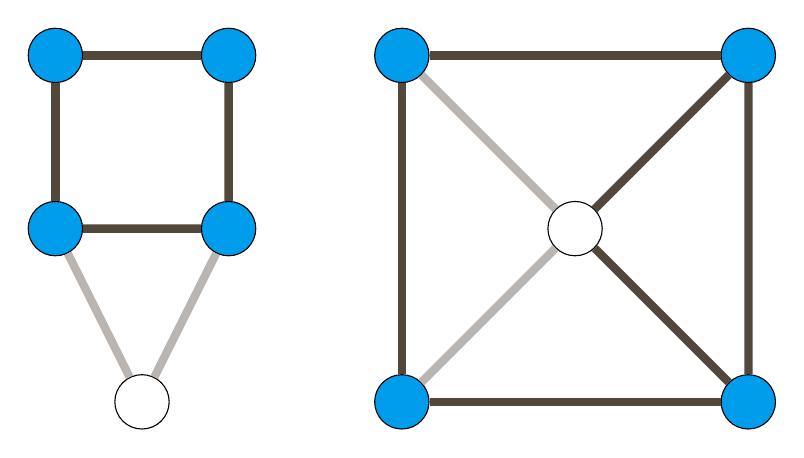
\begin{tikzpicture}[scale=1.1]%{{{
        \node[draw, circle, fill=uofgcobalt, inner sep=5pt, font=\bfseries] (Na) at (0,  0)
        {\vphantom{0}};
        \node[draw, circle, fill=uofgcobalt, inner sep=5pt, font=\bfseries] (Nb) at (0, -2)
        {\vphantom{0}};
        \node[draw, circle, fill=uofgcobalt, inner sep=5pt, font=\bfseries] (Nc) at (2, 0)
        {\vphantom{0}};
        \node[draw, circle, fill=uofgcobalt, inner sep=5pt, font=\bfseries] (Nd) at (2, -2)
        {\vphantom{0}};
        \node[draw, circle, fill=white, inner sep=5pt, font=\bfseries] (Ne) at (1, -4) 
        {\vphantom{0}};

        \draw [edge] (Na) -- (Nb);
        \draw [edge] (Na) -- (Nc);
        \draw [edge] (Nb) -- (Nd);
        \draw [edge] (Nc) -- (Nd);
        \draw [ledge] (Nb) -- (Ne);
        \draw [ledge] (Nd) -- (Ne);

        \node[draw, circle, fill=uofgcobalt, inner sep=5pt, font=\bfseries] (N1) at (4,  0) {\vphantom{0}};
        \node[draw, circle, fill=uofgcobalt, inner sep=5pt, font=\bfseries] (N2) at (4,  -4) {\vphantom{0}};
        \node[draw, circle, fill=white, inner sep=5pt, font=\bfseries] (N3) at (6, -2) {\vphantom{0}};
        \node[draw, circle, fill=uofgcobalt, inner sep=5pt, font=\bfseries] (N4) at (8, 0) {\vphantom{0}};
        \node[draw, circle, fill=uofgcobalt, inner sep=5pt, font=\bfseries] (N5) at (8, -4) {\vphantom{0}};

        \draw [edge] (N1) -- (N2);
        \draw [ledge] (N1) -- (N3);
        \draw [edge] (N1) -- (N4);
        \draw [ledge] (N2) -- (N3);
        \draw [edge] (N2) -- (N5);
        \draw [edge] (N3) -- (N4);
        \draw [edge] (N3) -- (N5);
        \draw [edge] (N4) -- (N5);

   \end{tikzpicture}\end{center}
\end{wrapfigure}

The \textbf{maximum common subgraph problem} is to find the largest graph which is isomorphic to
a subgraph of two graphs simultaneously---the size of the maximum common subgraph gives us a measure of how similar two graphs are.

\bigskip

In the induced variant of subgraph isormorphism when a pattern cannot be found in a target graph, we may seek a result which maps as many vertices of the pattern into the target as possible.  This is precisely the maximum common subgraph problem.

\bigskip

The maximum common subgraph problem is much more difficult in practice than subgraph isomorphism.
The state of the art for the maximum common subgraph
problem becomes \textbf{computationally
infeasible at only 35 vertices} when working with
unlabelled graphs. This is largely because strong inference,
based upon the degrees of vertices and the
distances or paths between them, is possible with subgraph isomorphism,
but not maximum common subgraph.}

\column{0.5}

\block{$k$-less Subgraph Isomorphism (Most of a Pattern)}{

A \textbf{$k$-less subgraph isomorphism} between a pattern and target graph, is a subgraph isomorphism
where we seek a mapping from all but $k$ verticies of the pattern to the target.

\bigskip

If $k$ is reasonably small, weakened forms of invariants from subgraph isomorphism (based on vertex degrees and paths) are still effective at reducing the search space.  In the example, upon removal of the central vertex from the pattern, we have a $1$-less isomorphism from the pattern to the target.

\bigskip

\begin{center}
    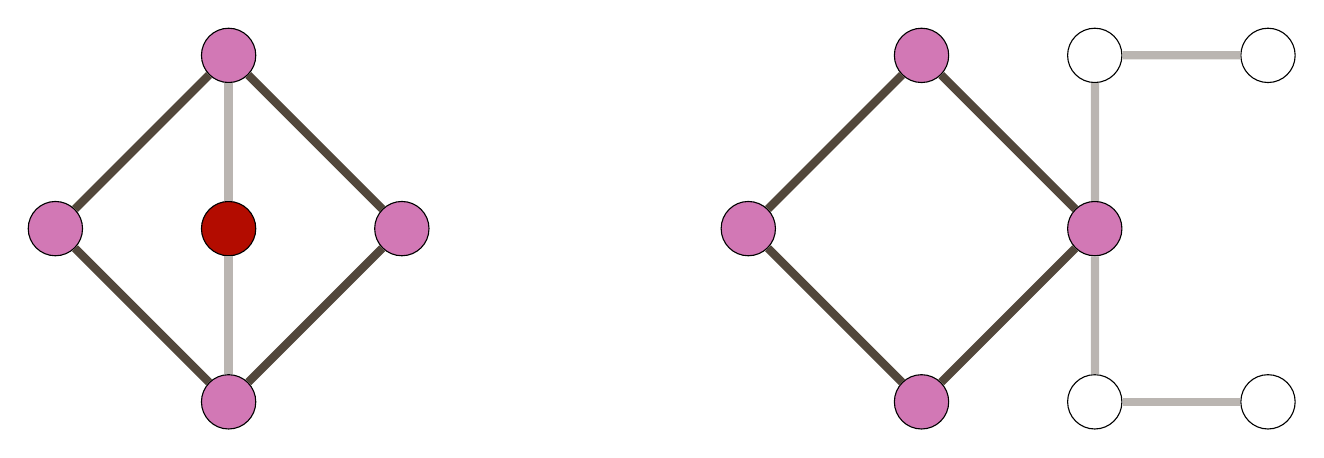
\begin{tikzpicture}[scale=1.1]%[every node/.style={circle, inner sep=0.5mm,node
        %distance=10mm,fill=black}, scale=0.2]

        \node[draw, circle, fill=uofgrose, inner sep=5pt, font=\bfseries] (d) at (0,0) {\vphantom{0}}; 
        \node[draw, circle, fill=uofgrose, inner sep=5pt, font=\bfseries]  (a) at (-2,2){\vphantom{0}}; 
        \node[draw, circle, fill=uofgpillarbox, inner sep=5pt, font=\bfseries]  (c) at (0,2) {\vphantom{0}}; 
        \node[draw, circle, fill=uofgrose, inner sep=5pt, font=\bfseries]  (e) at (2,2) {\vphantom{0}}; 
        \node[draw, circle, fill=uofgrose, inner sep=5pt, font=\bfseries]  (b) at (0,4) {\vphantom{0}}; 

        \draw[edge] (a) -- (b);
        \draw[edge] (a) -- (d);
        \draw[edge] (b) -- (e);
        \draw[ledge] (b) -- (c);
        \draw[ledge] (c) -- (d);
        \draw[edge] (d) -- (e);

        \node[draw, circle, fill=uofgrose, inner sep=5pt, font=\bfseries] (f) at (8,0) {\vphantom{0}};
        \node[draw, circle, fill=uofgrose, inner sep=5pt, font=\bfseries] (g) at (6,2) {\vphantom{0}};
        \node[draw, circle, fill=white, inner sep=5pt, font=\bfseries] (h) at (10,4) {\vphantom{0}};
        \node[draw, circle, fill=uofgrose, inner sep=5pt, font=\bfseries] (i) at (10,2) {\vphantom{0}};
        \node[draw, circle, fill=uofgrose, inner sep=5pt, font=\bfseries] (j) at (8,4) {\vphantom{0}};
        \node[draw, circle, fill=white, inner sep=5pt, font=\bfseries] (k) at (10,0) {\vphantom{0}};
        \node[draw, circle, fill=white, inner sep=5pt, font=\bfseries] (l) at (12,0){\vphantom{0}};
        \node[draw, circle, fill=white, inner sep=5pt, font=\bfseries] (m) at (12,4) {\vphantom{0}};

        \draw[edge] (f) -- (i);
        \draw[edge] (g) -- (f);
        \draw[edge] (i) -- (j);
        \draw[edge] (g) -- (j);
        \draw[ledge] (h) -- (m);
        \draw[ledge] (h) -- (i);
        \draw[ledge] (i) -- (k);
        \draw[ledge] (k) -- (l);   
        %\path[solid] (a) edge (b) edge (d)
        %    (e) edge (b) edge (d)
        %    (d) edge (c) edge (f)
        %    (c) edge (h)
        %    (f) edge (g);
    \end{tikzpicture}
\end{center}
\bigskip

Are there instances for which $k = 0$ is unsatisfiable, but that
are satisfiable for small $k$? For the problem families which
do not consist entirely of satisfiable instances, we plot this for both the induced and non-induced variants.
\vspace*{1.48cm}
\bigskip
\begin{center}
\input{gen-graph-which-k-by-family}
\end{center}
\bigskip
\vspace*{1.46cm}
In the ``phase'' family, which consists of instances
crafted to be extremely difficult to solve, we are not able
to answer this question, and in the ``scalefree'' family we
see no satisfiable instances with low but not zero $k$. 

\bigskip

However, in several of the remaining families our algorithm manages to provide exact solutions for many instances. This is particularly
interesting for the ``images-CVIU11'', where the size of the solution has a
direct \textbf{real-world interpretation} in terms of \textbf{closeness of image
matching}.

}

\end{columns}

\block{Maximum Common Subgraph: Solving from the Top Down}{

\begin{wrapfigure}[13]{r}{0.66\linewidth}
\begin{center}
\input{gen-graph-runtimes}
\end{center}
\end{wrapfigure}
What would happen if we used the $k$-less approach to solve the
maximum common induced problem? We could simply start
at $k = 0$, and increase $k$ until a solution is found. This \textbf{tackles the problem in the opposite direction to existing
approaches}, which work by attempting to construct
larger and larger solutions. In the figure, ``$k\downarrow$'' is our algorithm, whilst ``FC'' and
``clique'' are state of the art maximum common subgraph algorithms. 

\bigskip

We see that \textbf{our approach is able to close over twice
as many of these instances as the previous state of the art}---which struggles due to its RAM requirements.
On instances designed for the maximum subgraph problem we are still the single strongest solvers, and our performance tends to be complementary to that of the clique encoding.
}
\begin{columns}
\column{0.5}

\block{See the Paper for\ldots}{
    \begin{itemize}
        \item ~ Description of our new invariants, and proofs that they hold. 
        \item ~ Description of the algorithm.
    \end{itemize}
}

\column{0.5}

\block{Future Work}{
Develop an algorithm for maximum common subgraph which makes use of an upper bound from our approach and a lower bound from the clique approach, stopping when the bounds converge.
}

\end{columns}

{
    \colorlet{blockbodybgcolor}{uofgsandstone!80!white}
    \colorlet{blocktitlebgcolor}{uofgsandstone!80!white}
    \block[bodyverticalshift=1.2cm]{}{
        This work was supported by the Engineering and Physical Sciences Research Council [grant
        numbers EP/K503058/1 and EP/M506539/1]. \hfill \texttt{\textcolor{white}{c.reilly.2@research.gla.ac.uk}}
    }
}

\end{document}

